\documentclass[a4paper,10pt,french,twocolumn]{scrartcl}
\usepackage{amsthm}
\usepackage{amsmath}
\usepackage[T1]{fontenc}
\usepackage{graphicx}
\usepackage{titlesec}
\usepackage{ulem}
\usepackage[dvipsnames]{xcolor}
\usepackage{color}
\usepackage{amssymb}
\usepackage{caption}
\usepackage[mathscr]{euscript}
\usepackage{babel} 
\usepackage{helvet} 
\usepackage[utf8]{inputenc}
\usepackage[T1]{fontenc}
\usepackage{geometry}
\usepackage{pgfplots}
\pgfplotsset{compat=1.15}
\usepackage{mathrsfs}
\DeclareMathOperator{\e}{e}
\usetikzlibrary{arrows}
\title{La fonction exponentielle : Correction exercices}
\date{}
 \renewcommand*\familydefault{\sfdefault} 
\geometry{a4paper}
% -------------------------------------------------------------------------------------------------
% ----------- Création des commandes de couleur pour les titres ----------
% -------------------------------------------------------------------------------------------------
\newcommand{\sectionred}[1]{{\color{red}{\uuline{\color{black}#1}}}}
\newcommand{\sectiongreen}[1]{{\color{ForestGreen}{\uuline{\color{black}#1}}}}
\newcommand{\sectionblue}[1]{{\color{NavyBlue}{\uuline{\color{black}#1}}}}
\begin{document}
\maketitle
% -------------------------------------------------------------------------------------------------
% ---------------- Modification des titres de niveau 1,2 et 3 --------------------
% -------------------------------------------------------------------------------------------------
\titleformat
{\section} % command
%[display] % shape
{\Large} % format
{{\color{red}\uuline{\color{black}\thesection -}}} % label
{0ex} % sep
{\sectionred} % before-code
[] % after-code

\titleformat
{\subsection}%[display] % shape
{\Large} % format
{{\color{ForestGreen}\uuline{\color{black}\thesubsection -}}} % label
{0ex} % sep
{\sectiongreen} % before-code
[] % after-code

\titleformat
{\subsubsection} % command
%[display] % shape
{\large} % format
{{\color{NavyBlue}\uuline{\color{black}\thesubsubsection -}}} % label
{0ex} % sep
{\sectionblue} % before-code
[] % after-code

% -------------------------------------------------------------------------------------------------
% ---------------- Début du corps du document ------------------------------------
% -------------------------------------------------------------------------------------------------
\section{Exercice\:86\:page\:156}
a) La fonction $g$ est d\'erivable sur $R$.

Pour tout nombre r\'eel $x$,

$u(x) = 3 - x$ et $u'(x) = -1$

$v(x) = e^x$ et $v'(x) = e^x$

\bigbreak
$g'(x) = -1 \times e^x + (3 - x) \times e^x$

$g'(x) = e^x (-1 + 3 - x)$

$g'(x) = e^x (2 - x)$
\bigbreak
b)  Pour tout nombre réel $x$, $e^x > 0$, donc $g'(x)$ est du signe de $2 - x$.
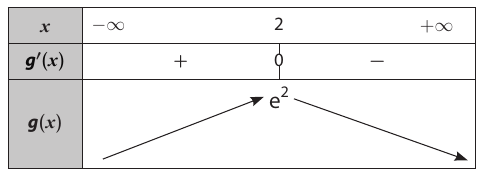
\includegraphics[scale=0.6]{ex1}
\bigbreak
c) Une équation de la tangente T au point
d’abscisse 0 est :

$y = g'(0)(x-0)+g(0)$

$y = \e^0(2-0)(x-0)+(3-0)\e^0$

$y = 2(x-0)+3$

$y = 2x+3$

\bigbreak
d)

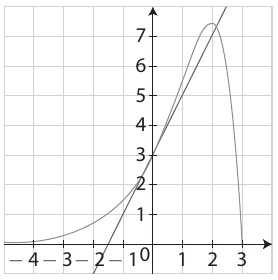
\includegraphics[scale=0.6]{ex2}

\section{Exercice\:87\:page\:156}
a) Les fonctions f et g sont dérivables sur R et
pour tout nombre réel x,

$u(x) = 2 - x$ et $u'(x) = - 1$

$v(x) = \e^x$ et $v'(x) = \e^x$

$f'(x) = -1 \times \e^x + (2 - x) \times \e^x$

$f'(x) = \e^x ( -1 + 2 - x)$

$f'(x) = \e^x ( 1 - x)$
\bigbreak
$u(x) = x2$ et $u'(x) = 2 x$

$v(x) = \e^x$ et $v'(x) = \e^x$

$g'(x) = 2x \times \e^x + x^2 \times \e^x$

$g'(x) = \e^x (x^2 + 2 x )$

\bigbreak
b) Pour tout nombre réel x, $\e^x > 0$, donc $f'(x)$ est du signe de $1- x$ et $g'(x)$ est du signe de $x^2 + 2x$.

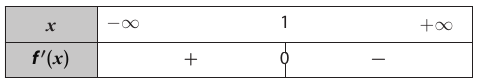
\includegraphics[scale=0.6]{ex3}

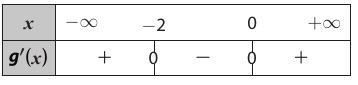
\includegraphics[scale=0.6]{ex4}

$x^2 + 2x =0$

$x(x+2) = 0$

\bigbreak

c) La fonction f est croissante sur l’intervalle $]- \infty ; 1]$.
La courbe 2 est donc celle de la fonction f et la courbe 1 est celle de la fonction g.
\end{document}
